\documentclass{article}
\usepackage[utf8]{inputenc}
\usepackage{amsmath} % For mathematical equations
\usepackage{amssymb} % For mathematical symbols
\usepackage{graphicx} % For including graphics (not strictly needed for this content, but good to have)
\usepackage{booktabs} % For professional-looking tables

\usepackage{pgfplots}
\pgfplotsset{compat=1.18}
\usepackage[T1]{fontenc}
\usepackage{caption}

\usepackage[left=1in,right=1in,top=1in,bottom=1in]{geometry} % Adjust margins

\begin{document}

\section*{Section 1 – Probability (6 pts)}

\begin{tabular}{p{0.05\textwidth} p{0.65\textwidth} l}
\toprule
\textbf{Q} & \textbf{Work} & \textbf{Answer} \\
\midrule
1 & P(TV or Online)=P(TV)+P(Online)-P(Both)=0.30+0.25-0.10=0.45 & \textbf{(B) 0.45} \\
2 & Conditional probability & \\
 & $=\dfrac{120+80}{120+80+50+50}= \dfrac{200}{300}=0.6667$ & \textbf{(D) 0.67} \\
\bottomrule
\end{tabular}

\vspace{1em} % Add some vertical space
\hrule % Horizontal line

\section*{Section 2 – Descriptive statistics (9 pts)}

\begin{center}
  \begin{minipage}[t]{0.30\textwidth}
    \centering
    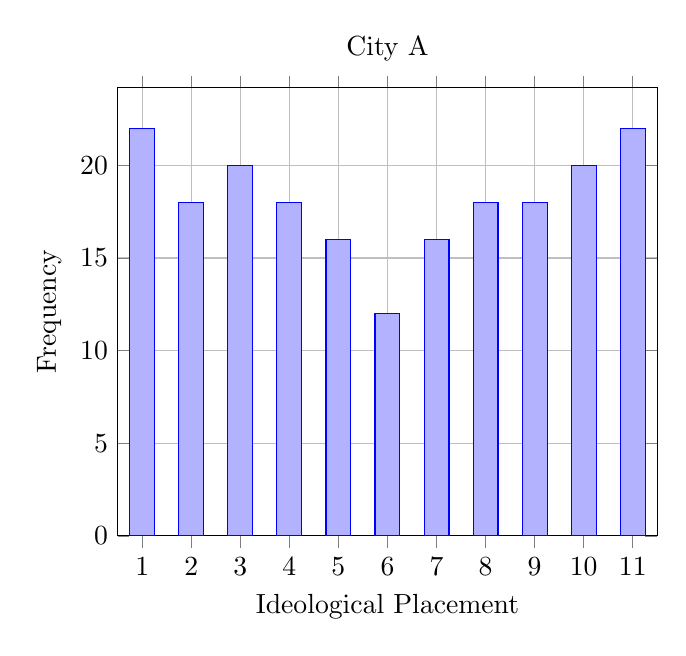
\begin{tikzpicture}
      \begin{axis}[
          ybar,
          bar width=9pt,
          ylabel={Frequency},
          xlabel={Ideological Placement},
          ymin=0,
          xtick=data,
          xticklabels={1,2,3,4,5,6,7,8,9,10,11},
          title={City~A},
          enlarge x limits=0.05,
          grid=major
        ]
        \addplot coordinates {(1,22) (2,18) (3,20) (4,18) (5,16) (6,12) (7,16) (8,18) (9,18) (10,20) (11,22)};
      \end{axis}
    \end{tikzpicture}
  \end{minipage}\hfill
  \begin{minipage}[t]{0.45\textwidth}
    \centering
    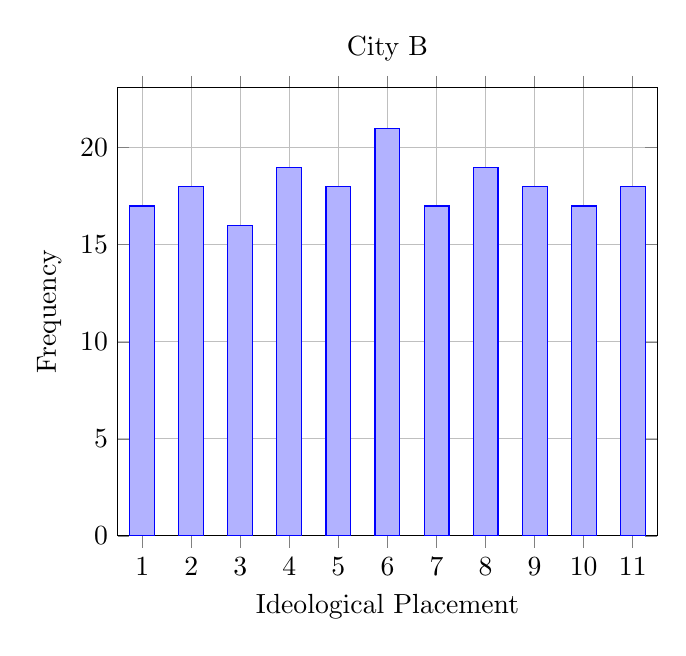
\begin{tikzpicture}
      \begin{axis}[
          ybar,
          bar width=9pt,
          ylabel={Frequency},
          xlabel={Ideological Placement},
          ymin=0,
          xtick=data,
          xticklabels={1,2,3,4,5,6,7,8,9,10,11},
          title={City~B},
          enlarge x limits=0.05,
          grid=major
        ]
        \addplot coordinates {(1,17) (2,18) (3,16) (4,19) (5,18) (6,21) (7,17) (8,19) (9,18) (10,17) (11,18)};
      \end{axis}
    \end{tikzpicture}
  \end{minipage}
\end{center}

1. \textbf{Shape comparison}
   \begin{itemize}
     \item \textit{City A} shows a clear \textbf{U-shaped/bimodal} pattern—peaks at the most-liberal (1) and most-conservative (11) ends, with a dip in the middle (score 6).
     \item \textit{City B} is \textbf{fairly uniform to mildly mound-shaped}, with a modest peak at the middle (score 6) and no dramatic tails.
   \end{itemize}

2. \textbf{Interpretation and comparison with mean and SD}

   Hence, even though the two cities share almost identical means ($\approx 6.0$) and similar SDs, their \textit{distributions} are very different.

3. \textbf{Main take-aways}
   \begin{itemize}
     \item \textit{City A}: electorate is polarized—many self-identify at ideological extremes, fewer at the center.
     \item \textit{City B}: views are more evenly spread, slightly concentrated around the center, suggesting a less-polarized public.
   \end{itemize}

\vspace{1em} % Add some vertical space
\hrule % Horizontal line

\section*{Section 3 – Random variables (5 pts)}

1. $E[C]=0(0.70)+5{,}000(0.20)+20{,}000(0.08)+100{,}000(0.02)=\$4{,}600$.

2. \textbf{Interpretation} – Over many years, an uninsured homeowner in this region would face an \textit{average} flood-damage bill of \$4,600 per year, even though most individual years cost \$0 and occasional years are far more expensive.

3. \textbf{Insurance decision} – Because \$4,000 $<$ \$4,600, the offered premium is below the long-run expected annual loss. Thus, given the provided decision rule, such homeowner would indeed take the insurance.

\vspace{1em} % Add some vertical space
\hrule % Horizontal line

\section*{Section 4 – Hypothesis testing (25 pts)}

1. \textbf{Hypotheses}
$$
H_0:\;p_{\text{FB}}-p_{\text{USB}}=0 \qquad
H_a:\;p_{\text{FB}}-p_{\text{USB}}\neq 0
$$

2. \textbf{Two-proportion $z$-test}
$$
\begin{aligned}
\hat p_1&=\frac{348}{600}=0.58,\;
\hat p_2=\frac{700}{1400}=0.50\\[2pt]
\hat p&=\frac{348+700}{600+1400}=0.524\\[4pt]
SE&=\sqrt{\hat p(1-\hat p)\Bigl(\frac1{600}+\frac1{1400}\Bigr)}=0.02437\\[4pt]
z&=\frac{\hat p_1-\hat p_2}{SE}=\frac{0.08}{0.02437}=3.2828
\end{aligned}
$$
Critical value at $\alpha = 0.05$ (two-tailed): $\pm1.96$.
Because $|z| = 3.283 > 1.96$, \textbf{reject $H_0$}.

3. \textbf{Plain-language conclusion} – There is strong statistical evidence (p < 0.01) that U.S. adults with foreign-born parents differ from those with U.S.-born parents in liking spicy food; the data suggest the former are more likely to enjoy it.

\vspace{1em} % Add some vertical space
\hrule % Horizontal line

\section*{Section 5 – Inference concepts (30 pts)}

\begin{tabular}{p{0.05\textwidth} p{0.15\textwidth} p{0.70\textwidth}}
\toprule
\textbf{Q} & \textbf{Correct choice} & \textbf{Reason} \\
\midrule
1 & \textbf{(B)} & Mid-point of CI is the sample estimate. \\
2 & \textbf{(D)} & 0.62 $\pm$ 1.96 $\times$ 0.019 = (0.5828, 0.6572) $\approx$ (58.3 \%, 65.7 \%). \\
3 & \textbf{(B)} & Hypotheses must compare population means $\mu_1,\mu_2$. We always write the null as $H_0 : \mu_1=\mu_2$. \\
\bottomrule
\end{tabular}

\vspace{1em} % Add some vertical space
\hrule % Horizontal line

\section*{Section 6 – Confidence intervals (25 pts)}

1. \textbf{Descriptive statistics}
$$
\bar x=\frac{29}{10}=2.9000,\qquad
s=\sqrt{\frac{\sum(x_i-\bar x)^2}{n-1}}=1.1972
$$

2. \textbf{99 \% $t$-interval}
$$
\begin{aligned}
n&=10,\;df=9,\;t_{0.005,9}=3.2498\\[2pt]
SE&=\frac{s}{\sqrt{n}}=\frac{1.1972}{\sqrt{10}}=0.3786\\[2pt]
ME&=t\,SE=3.2498(0.3786)=1.2304\\[4pt]
\text{CI}&=\bar x\pm ME=(2.9000\pm1.2304) \\
&=(1.6696,\;4.1304)
\end{aligned}
$$

3. \textbf{Interpretation} – We are 99 \% confident that the true average employee drinks between \textbf{about 1.7 and 4.1 cups} of coffee per workday. If we repeatedly took samples of 10 employees and built such intervals, about 99 \% of them would contain the true company-wide mean.

\end{document}
